\documentclass[10pt]{article}

\usepackage{mathtools}  % need for math tools
\usepackage{amsmath}    % need for subequations
\usepackage{graphicx}   % need for figures
\usepackage{verbatim}   % useful for program listings
\usepackage{color}      % use if color is used in text
\usepackage{subfigure}  % use for side-by-side figures
\usepackage{hyperref}   % use for hypertext links, including those to external documents and URLs
\usepackage{graphicx}   % Used to import the graphics

\setlength{\baselineskip}{16.0pt}   
\setlength{\parskip}{3pt plus 2pt}
\setlength{\parindent}{20pt}
\setlength{\oddsidemargin}{0.5cm}
\setlength{\evensidemargin}{0.5cm}
\setlength{\marginparsep}{0.75cm}
\setlength{\marginparwidth}{2.5cm}
\setlength{\marginparpush}{1.0cm}
\setlength{\textwidth}{150mm}



\begin{document}

\begin{center}
{\large Exercise 1} \\
\copyright 2012 by Arya Farahi \\
Jan 8, 2012
\end{center}

\section{Exercise 2.1 (FP addition is not associative)}

if we choose $X = 28.4762$, $Y = 3.5861$, $Z = 2.0624$ then for $ m = 3 $ we have:

\begin{equation}
 \overline{\overline{ ( \overline{X} + \overline{Y} ) } + \overline{Z} } = \overline{\overline{28.4 + 3.58} + 2.06} = \overline{31.9 + 2.06} = 33.9   
\end{equation}

and
  
\begin{equation}
 \overline{ \overline{X} + \overline{ ( \overline{Y} + \overline{Z} ) } } = \overline{28.4 + \overline{3.58 + 2.06}} = \overline{28.4 + 5.64} = 34.0   
\end{equation}

so FP numbers is not associative.


\section{Exercise 2.2 (An unstable Calculation)}

For the 1st part of the question \\*
The relative error is :    44004832 \\*
and    \\*
The absolute error is :    3.0667727 \\

For the 2nd part of this question (When $X_n = 4^n$) the related sequence is : \\
\begin{equation}
 X_{n+1} = 5 X_n - 4 X_{n-1}   
\end{equation}
The relative error is :    0.0000000 \\*
and \\*
The absolute error is :    0.0000000 \\

For the first part the truncation error increas as n increasing but for the second part it is not increasing. So, there is not a big deviation from the real answer in the second part of the problem.\\

Absolute error and relative error can be used to measure accuracy and stability for simple problems which we know the analytical solutino. But when we do not know the analytical solution we are not able to calculate the absolute error and relative error.\\

\section{Exercise 3.1 (Finite-Difference Estiate of the Second Derivative)}

By teylor expansion we can derive the following equations:\\

\begin{equation}\label{eq:eq11}
 f(x_0+h) = f(x_0) + hf'(x_0) + h^2f''(x_0)/2 + h^3f'''(x_0)/6 + \mathcal{O}(h^4_o)  
\end{equation}

and\\

\begin{equation}\label{eq:eq22}
 f(x_0-h) = f(x_0) - hf'(x_0) + h^2f''(x_0)/2 - h^3f'''(x_0)/6 + \mathcal{O}(h^4_o)  
\end{equation}

Simply by adding the equation number \ref{eq:eq11} and \ref{eq:eq22} we can derive the following formula:\\


\begin{equation}
f''(x_0) = \frac{f(x_0+h) - 2f(x_0) + f(x_0-h)}{ h^2}  + \mathcal{O}(h^4_o)  
\end{equation}




\section{Exercise 3.2 (Second Derivative Estimate on non-equidistant Grids)}

By teylor expansion we can derive the following equations:\\

\begin{equation}\label{eq:eq1}
 f(x_0+h_2) = f(x_0) + h_2f'(x_0) + h_2^2f''(x_0)/2 + h_2^3f'''(x_0)/6 + \mathcal{O}(h^4_o)  
\end{equation}

and\\

\begin{equation}\label{eq:eq2}
 f(x_0-h_1) = f(x_0) - h_1f'(x_0) + h_1^2f''(x_0)/2 - h_1^3f'''(x_0)/6 + \mathcal{O}(h^4_o)  
\end{equation}

Simply by multiplying equation number \ref{eq:eq1} by $h_1$ and multiplying equation number \ref{eq:eq2} by $h_2$ and then adding them we can derive the following equation:\\

\begin{equation}\label{eq:eq3}
f''(x_0) = 2\frac{h_1f(x_0+h_2) - (h_1 + h_2)f(x_0) + h_2f(x_0-h_1)}{h_2 h_1 (h_1 + h_2)}  + \mathcal{O}(h^4_o)  
\end{equation}



\section{Exercise 3.3 (Convergence of a Finite-Difference Estimate)}

\begin{figure}[h]
  \begin{center}
    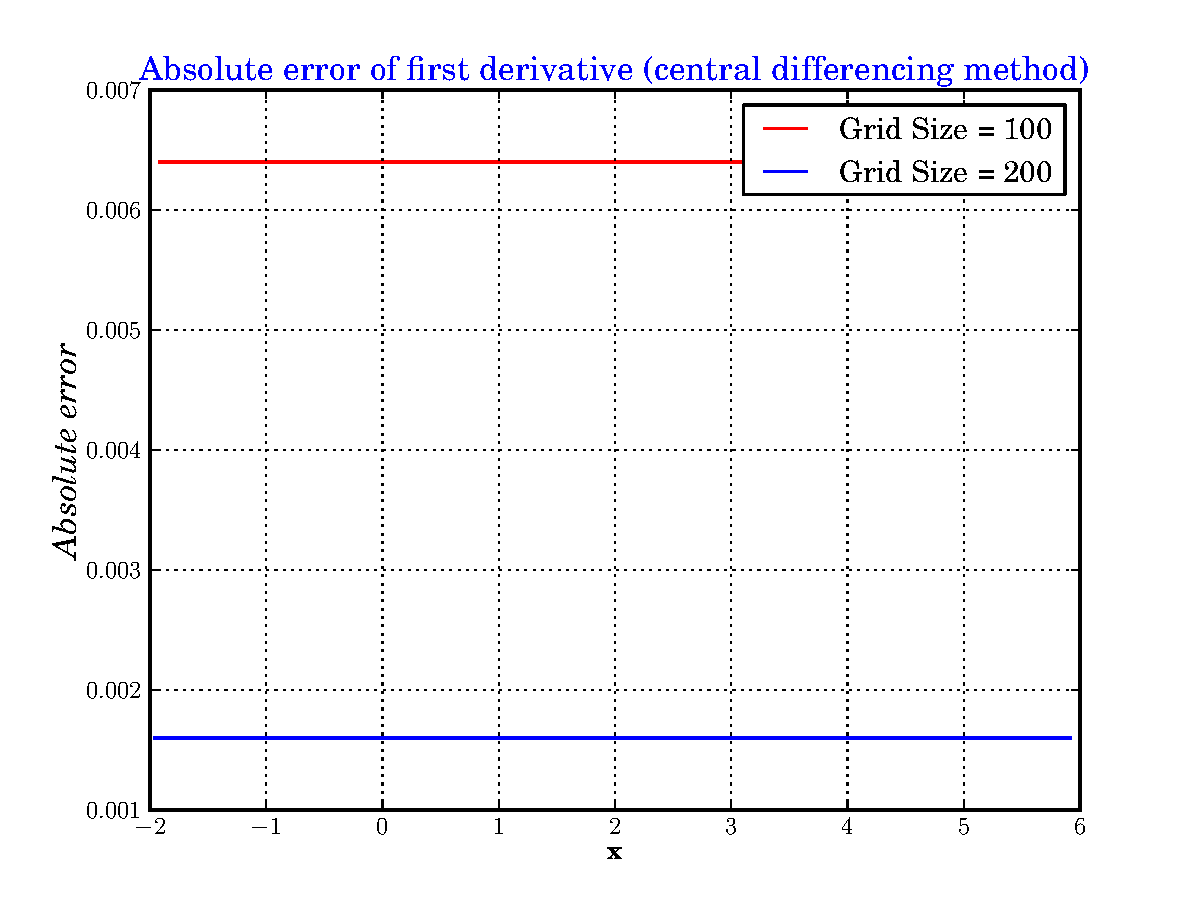
\includegraphics[totalheight=0.5\textheight]{plot1.pdf}
    \caption{\label{fig:ForwardMethod} Plot of the absolute error of first derivative with forward method for 200 and 100 cell grid size.}
  \end{center}
\end{figure}


\begin{figure}[h]
  \begin{center}
    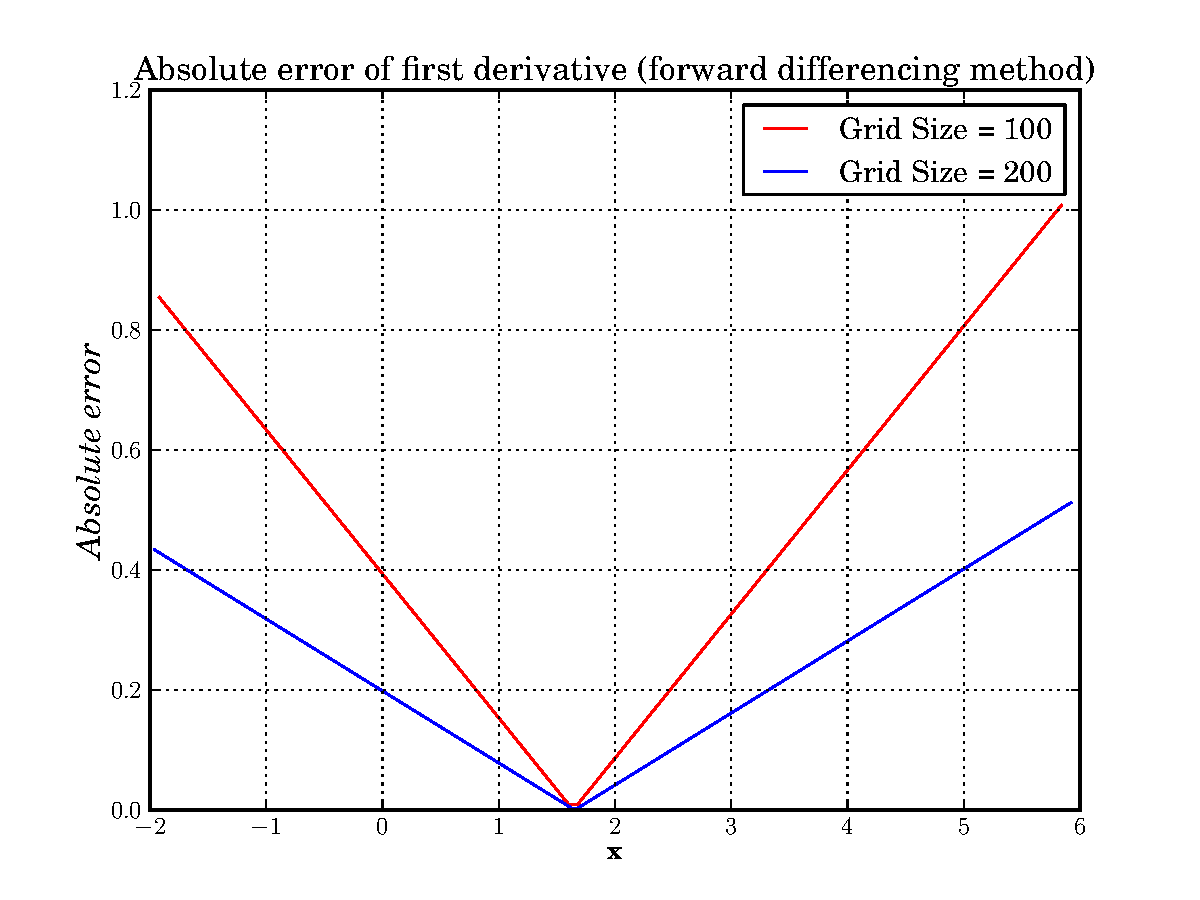
\includegraphics[totalheight=0.5\textheight]{plot2.pdf}
    \caption{\label{fig:CentralMethod} Plot of the absolute error of first derivative with forward method  with central method for 200 and 100 cell grid size.}
  \end{center}
\end{figure}

\begin{figure}[h]
  \begin{center}
    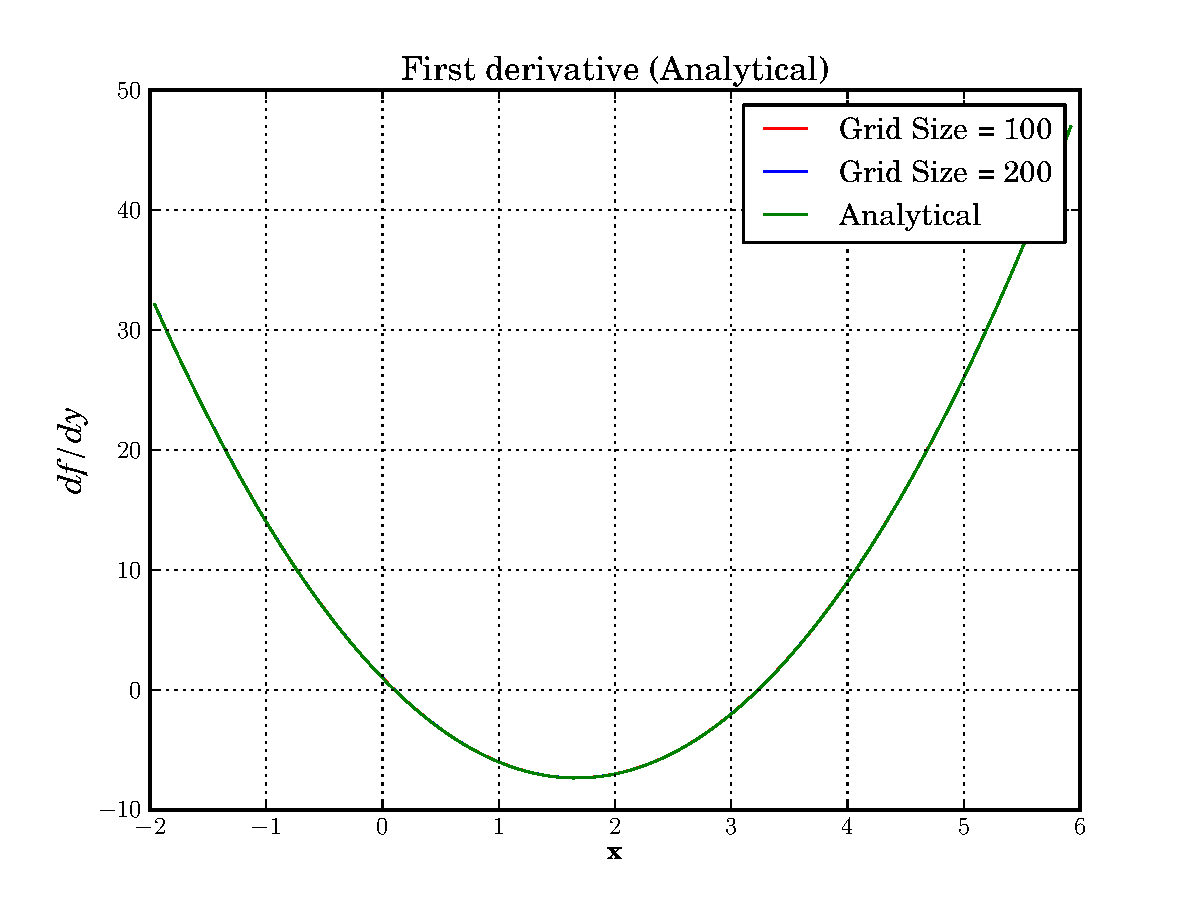
\includegraphics[totalheight=0.5\textheight]{plot3.pdf}
    \caption{\label{fig:ForwardMethoddf/dx} Plot of first derivative with forward method for 200 and 100 cell grid size.}
  \end{center}
\end{figure}


\begin{figure}[h]
  \begin{center}
    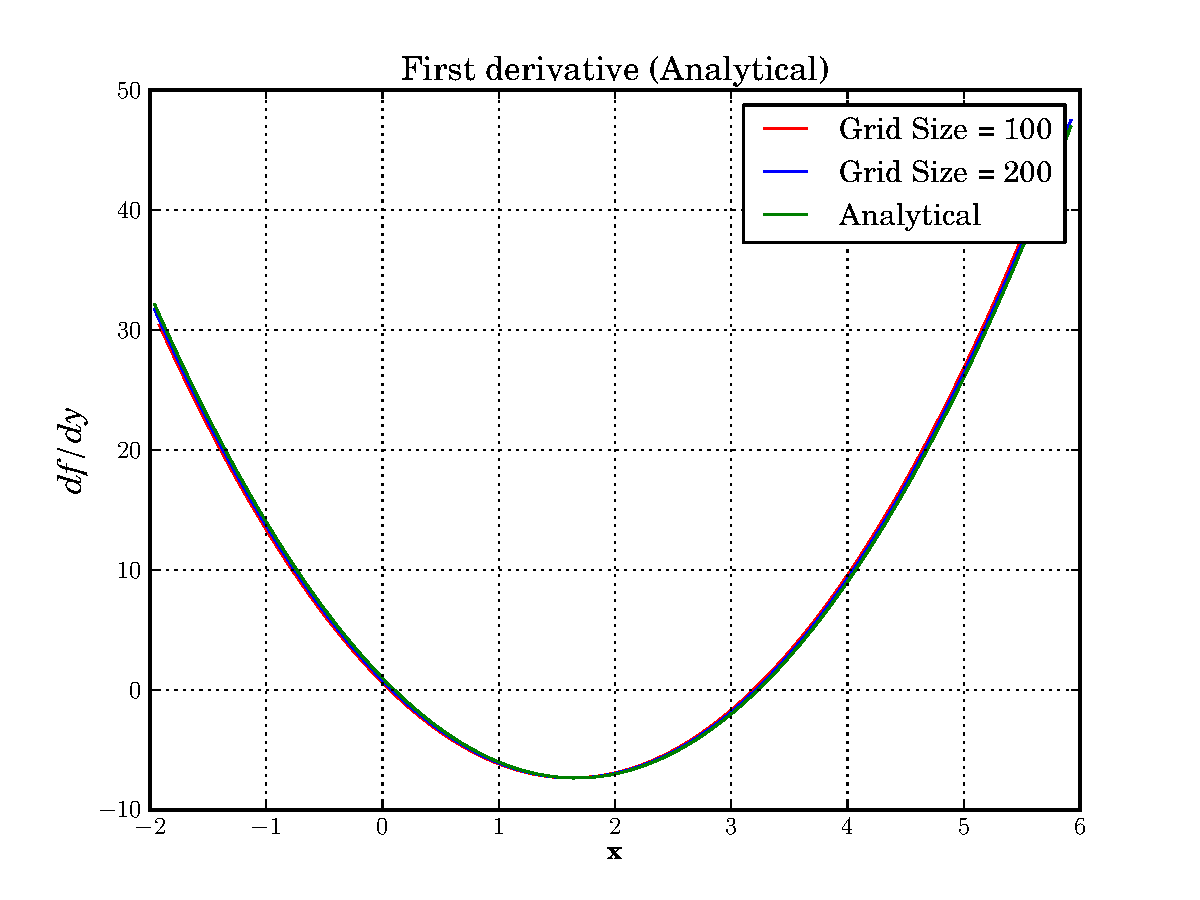
\includegraphics[totalheight=0.5\textheight]{plot4.pdf}
    \caption{\label{fig:CentralMethoddf/dx} Plot of first derivative with forward method with central method for 200 and 100 cell grid size.}
  \end{center}
\end{figure}

figure \ref{fig:ForwardMethod} showes the plot of absolute error of first derivative with forward method for two different grid size. (100 and 200 cell grid size) and figure \ref{fig:CentralMethod} showes the plot of absolute error of first derivative with central method for two different grid size. (100 and 200 cell grid size)


figure \ref{fig:ForwardMethoddf/dx} showes the plot of first derivative
 with forward method for two different grid size. (100 and 200 cell grid size) and figure \ref{fig:CentralMethoddf/dx} showes the plot of first derivative
with central method for two different grid size. (100 and 200 cell grid size)


As it is shown in the figure \ref{fig:ForwardMethod} and \ref{fig:CentralMethod} the absolute error for forward method get decreased with relation $\frac{(ABS-ERR)_1}{(ABS-ERR)_2} = \frac{1}{2}$ and for central method $\frac{(ABS-ERR)_1}{(ABS-ERR)_2} = \frac{1}{4}$  as we expected. So we can conclude that these methods converges to first derivative of our function.\\



\section{Exercise 4.1 (Runge’s Phenomenon)}

\begin{figure}[h]
  \begin{center}
    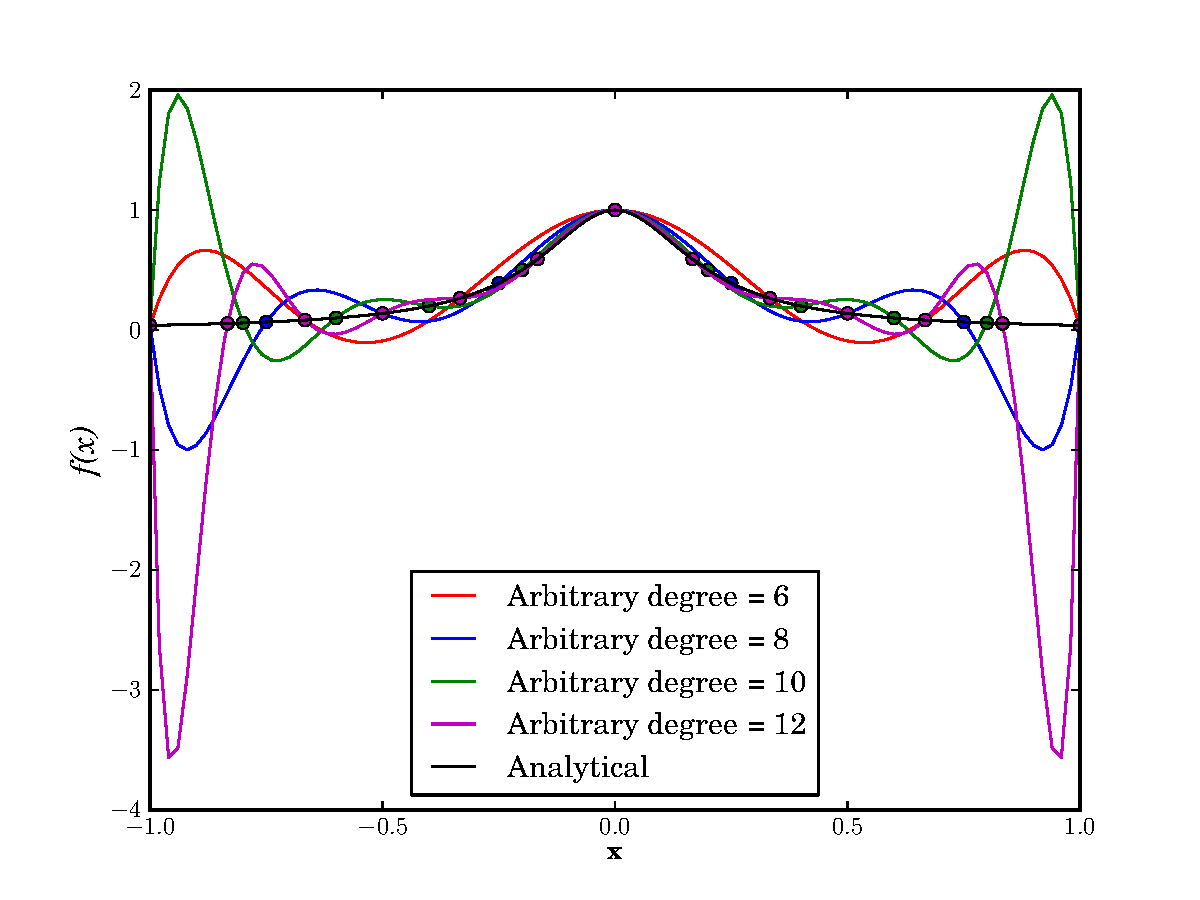
\includegraphics[totalheight=0.6\textheight]{plot5.pdf}
    \caption{\label{fig:Interpol} Runge’s phenomenon of non-convergence as exhibited by polynomials of degree 6, 8, 10, and 12 for the continuous function $f(x) = \frac{1}{(25x^2 + 1)}$ .}
  \end{center}
\end{figure}

Figure \ref{fig:Interpol} is Runge’s phenomenon of non-convergence as exhibited by polynomials of degree 6, 8, 10, and 12 for the continuous function $f(x) = \frac{1}{(25x^2 + 1)}$. And error norm-2 for cases n = 6, 8, 10, and 12 are equale to 8.30384118064, 9.63134306975, 12.9259174749, and 19.0058390679 respectivly.\\
  

\begin{figure}[h]
  \begin{center}
    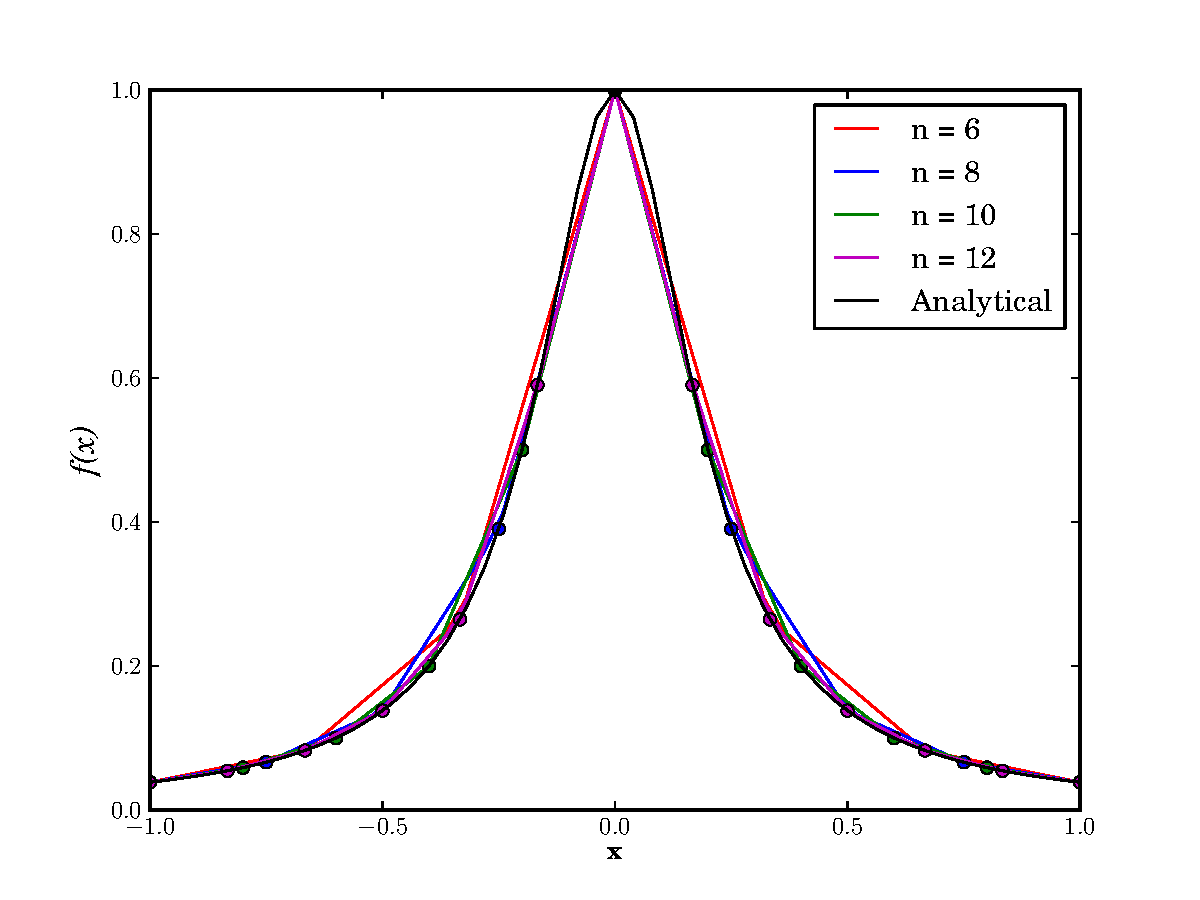
\includegraphics[totalheight=0.6\textheight]{plot6.pdf}
    \caption{\label{fig:Interpol2} is a linear interpolation with 6, 8, 10, and 12 points for the continuous function $f(x) = \frac{1}{(25x^2 + 1)}$ .}
  \end{center}
\end{figure}

Figure \ref{fig:Interpol2} is a linear interpolation with 6, 8, 10, and 12 points for the continuous function $f(x) = \frac{1}{(25x^2 + 1)}$. And error norm-2 for cases n = 6, 8, 10, and 12 are equale to 0.152684574991, 0.0748065476962, 0.0432249437241, and 0.0268469837336 respectivly.\\


\end{document}
